%% F1
\begin{figure*}[ht]
  \begin{subfigure}{.315\textwidth}
    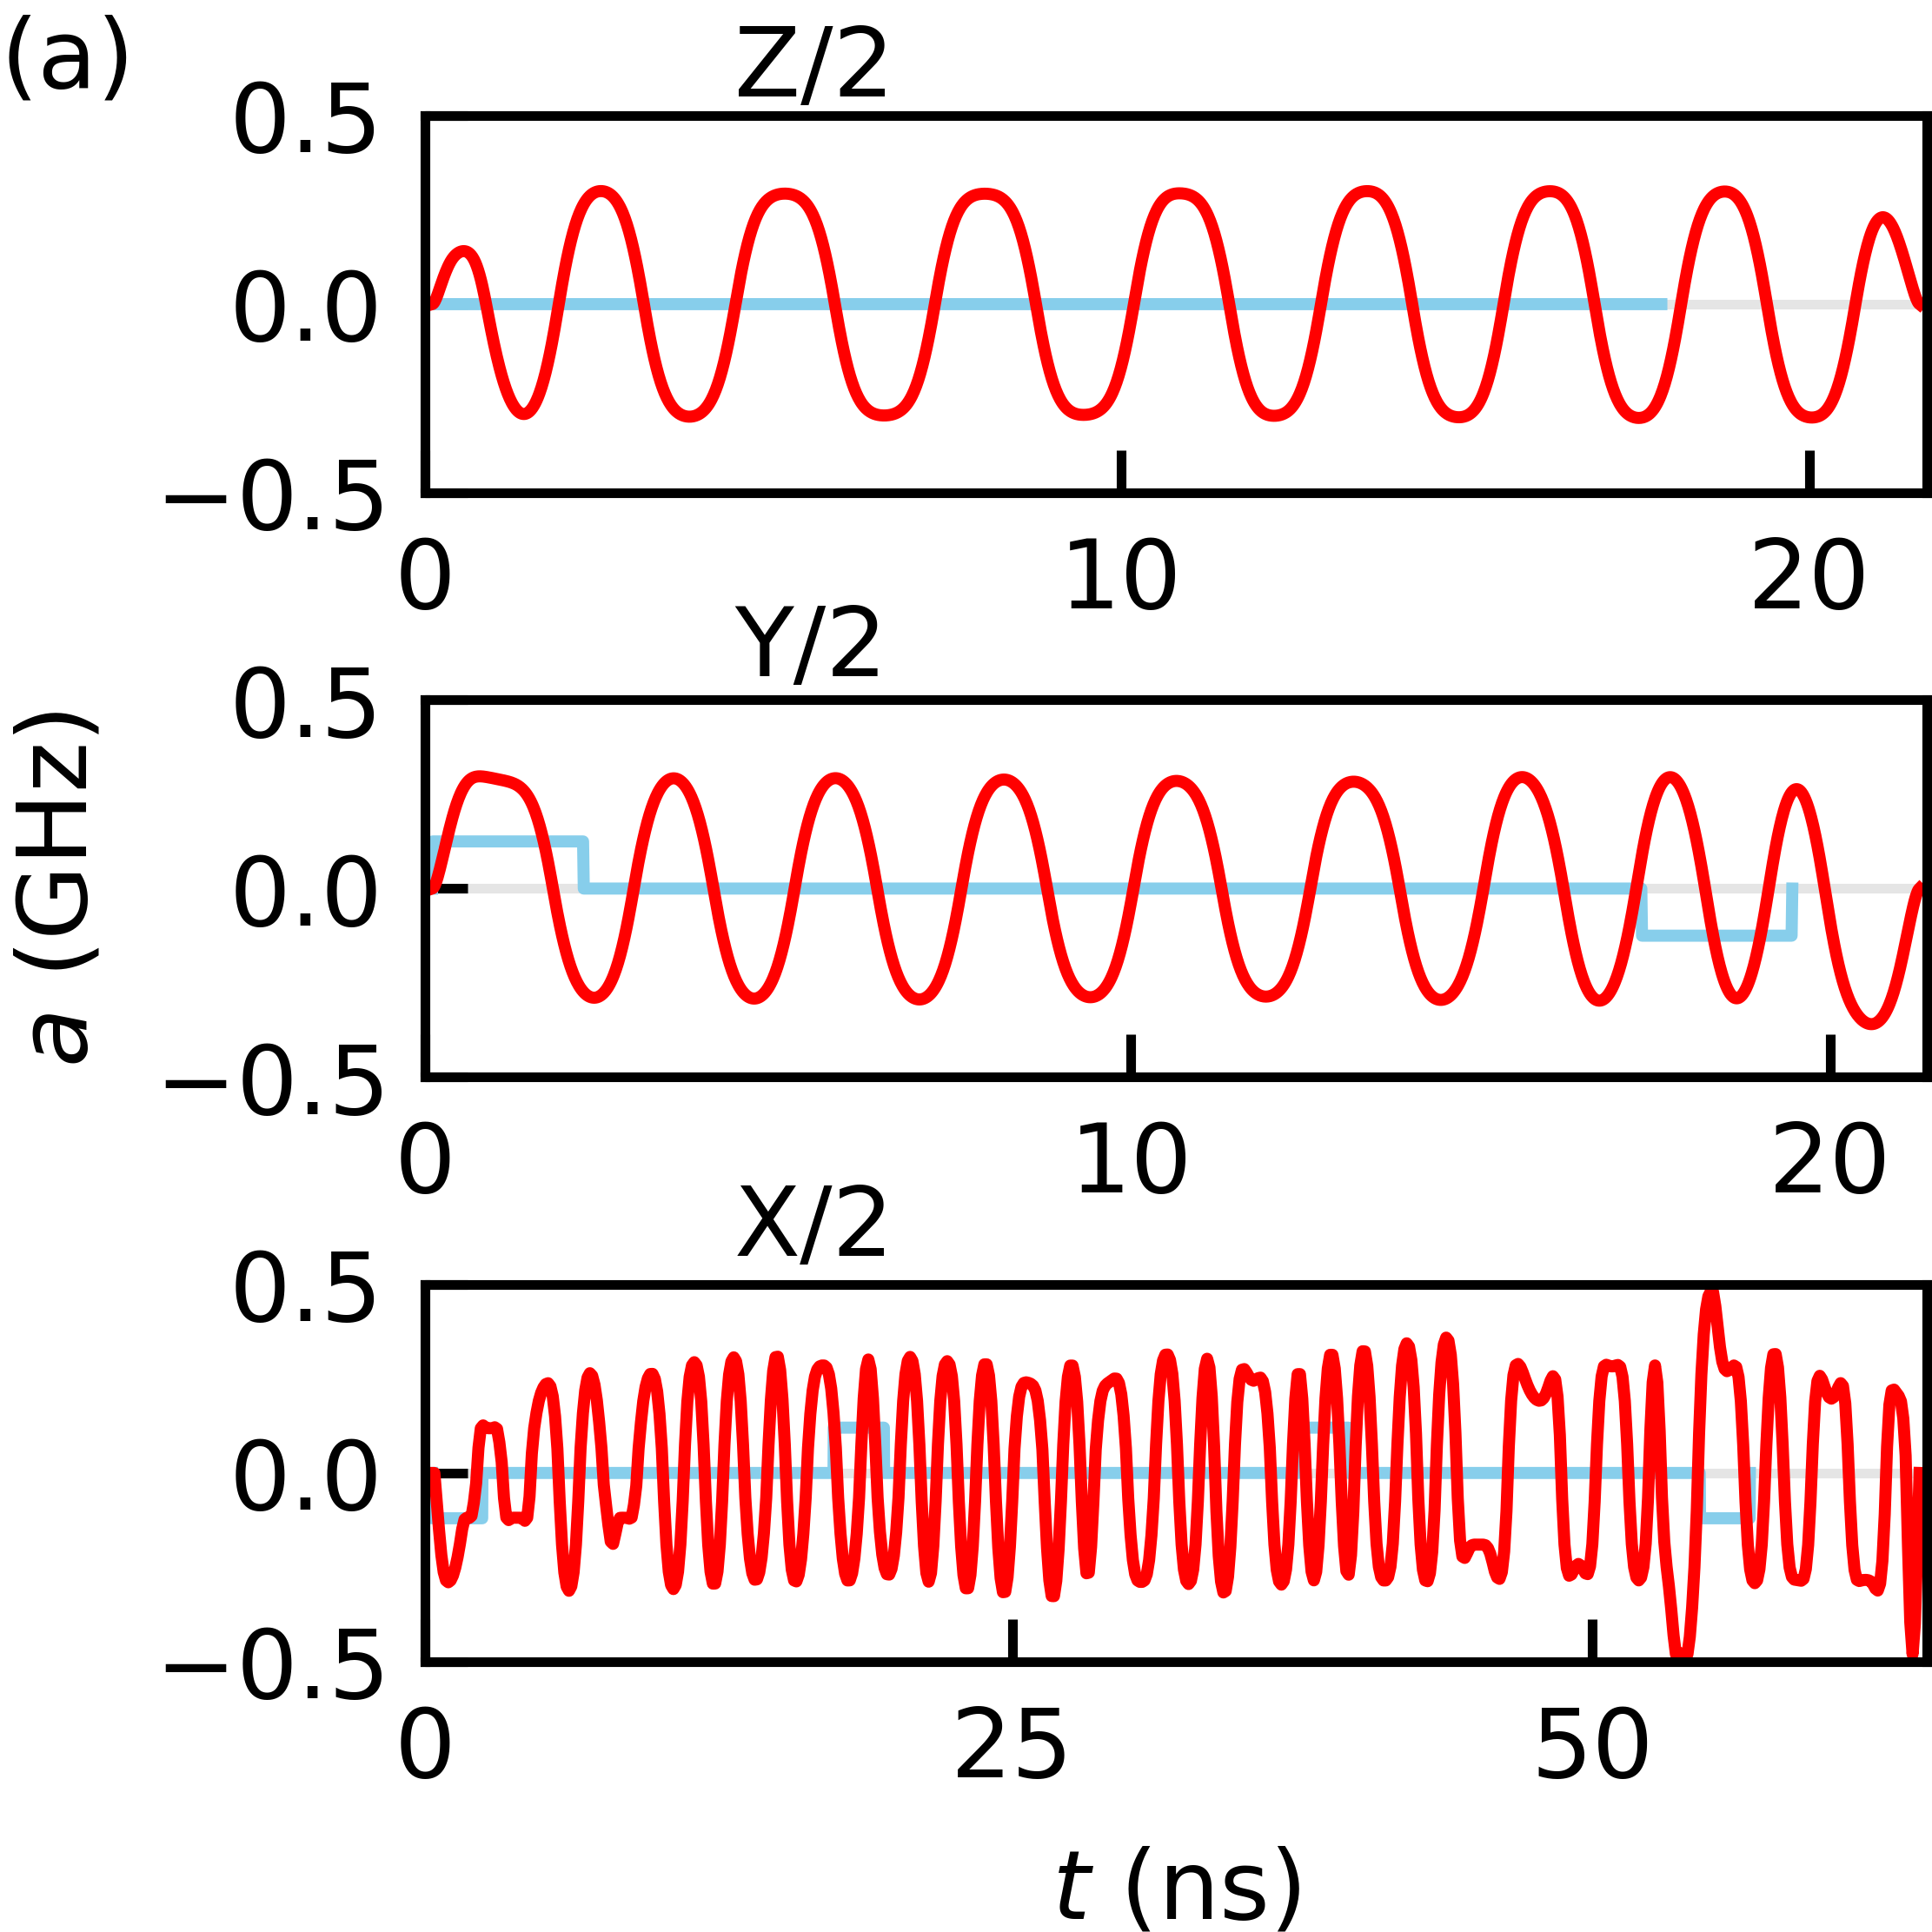
\includegraphics[width=\linewidth]{assets/f1a.png}
    \caption{\label{fig:longitudea}}
  \end{subfigure}\hfill
  \begin{subfigure}{.23\textwidth}
    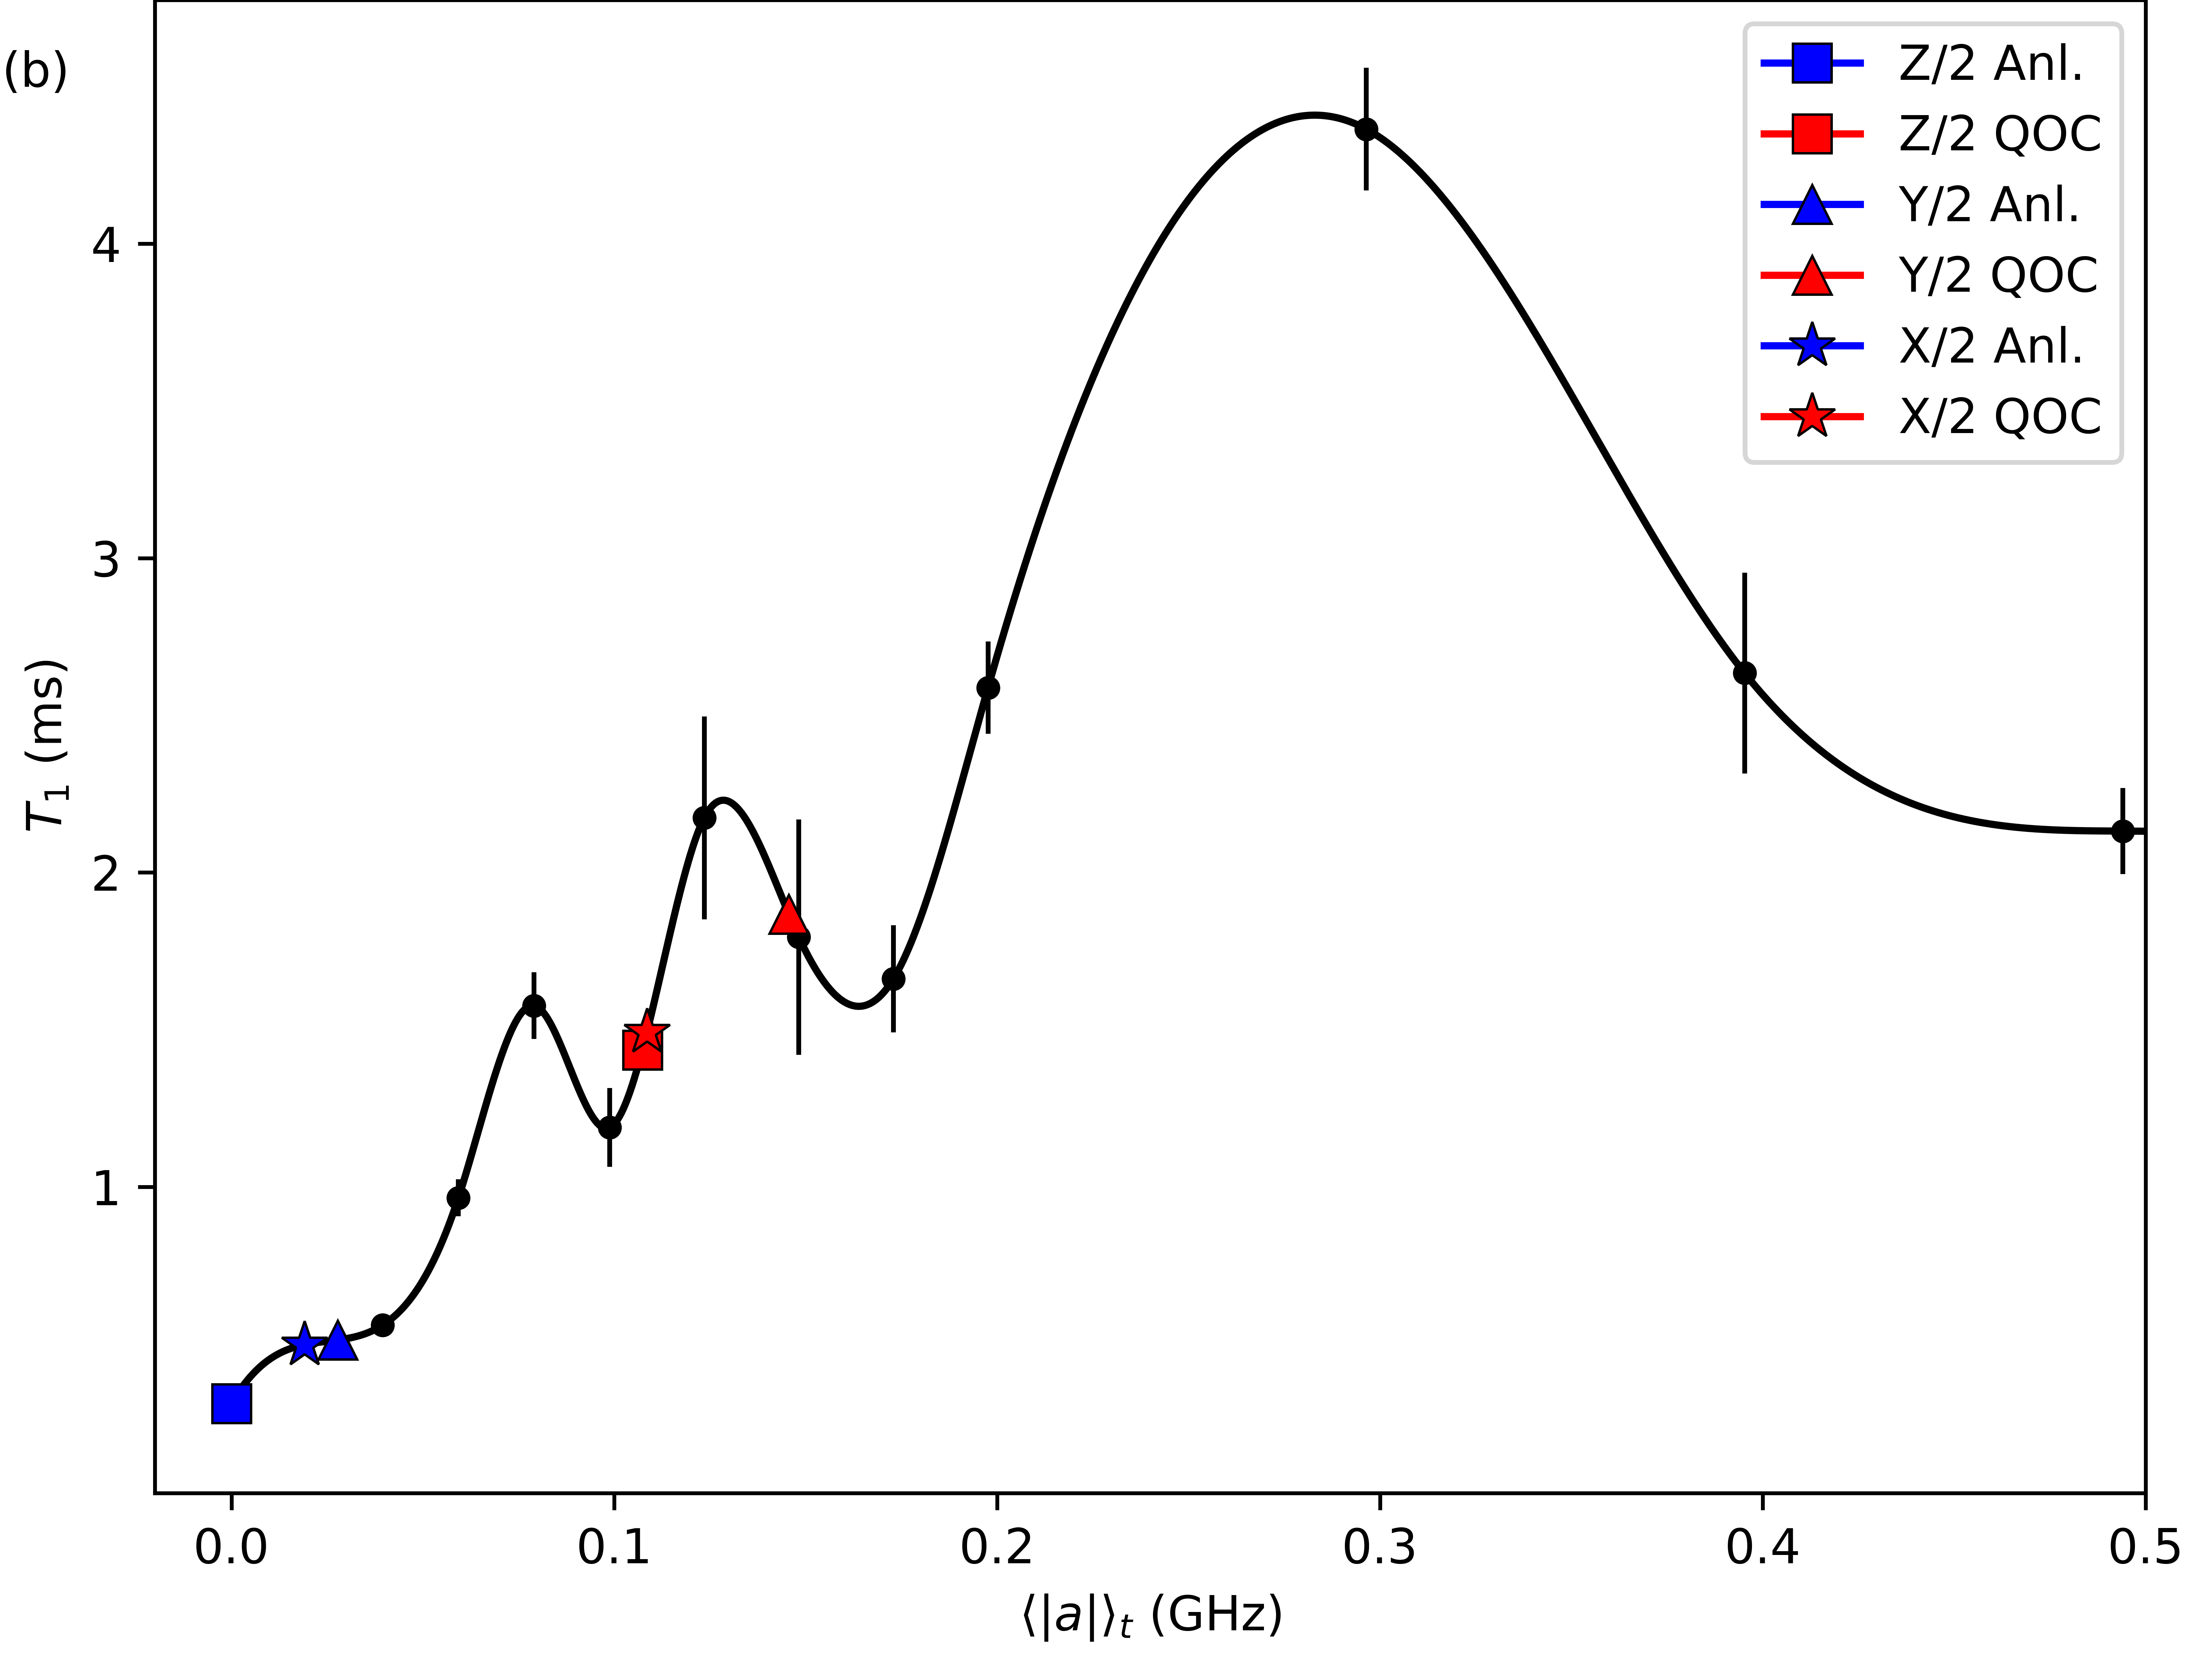
\includegraphics[width=\linewidth]{assets/f1b.png}
    \caption{\label{fig:longitudeb}}
  \end{subfigure}\hfill
  \begin{subfigure}{.4\textwidth}
    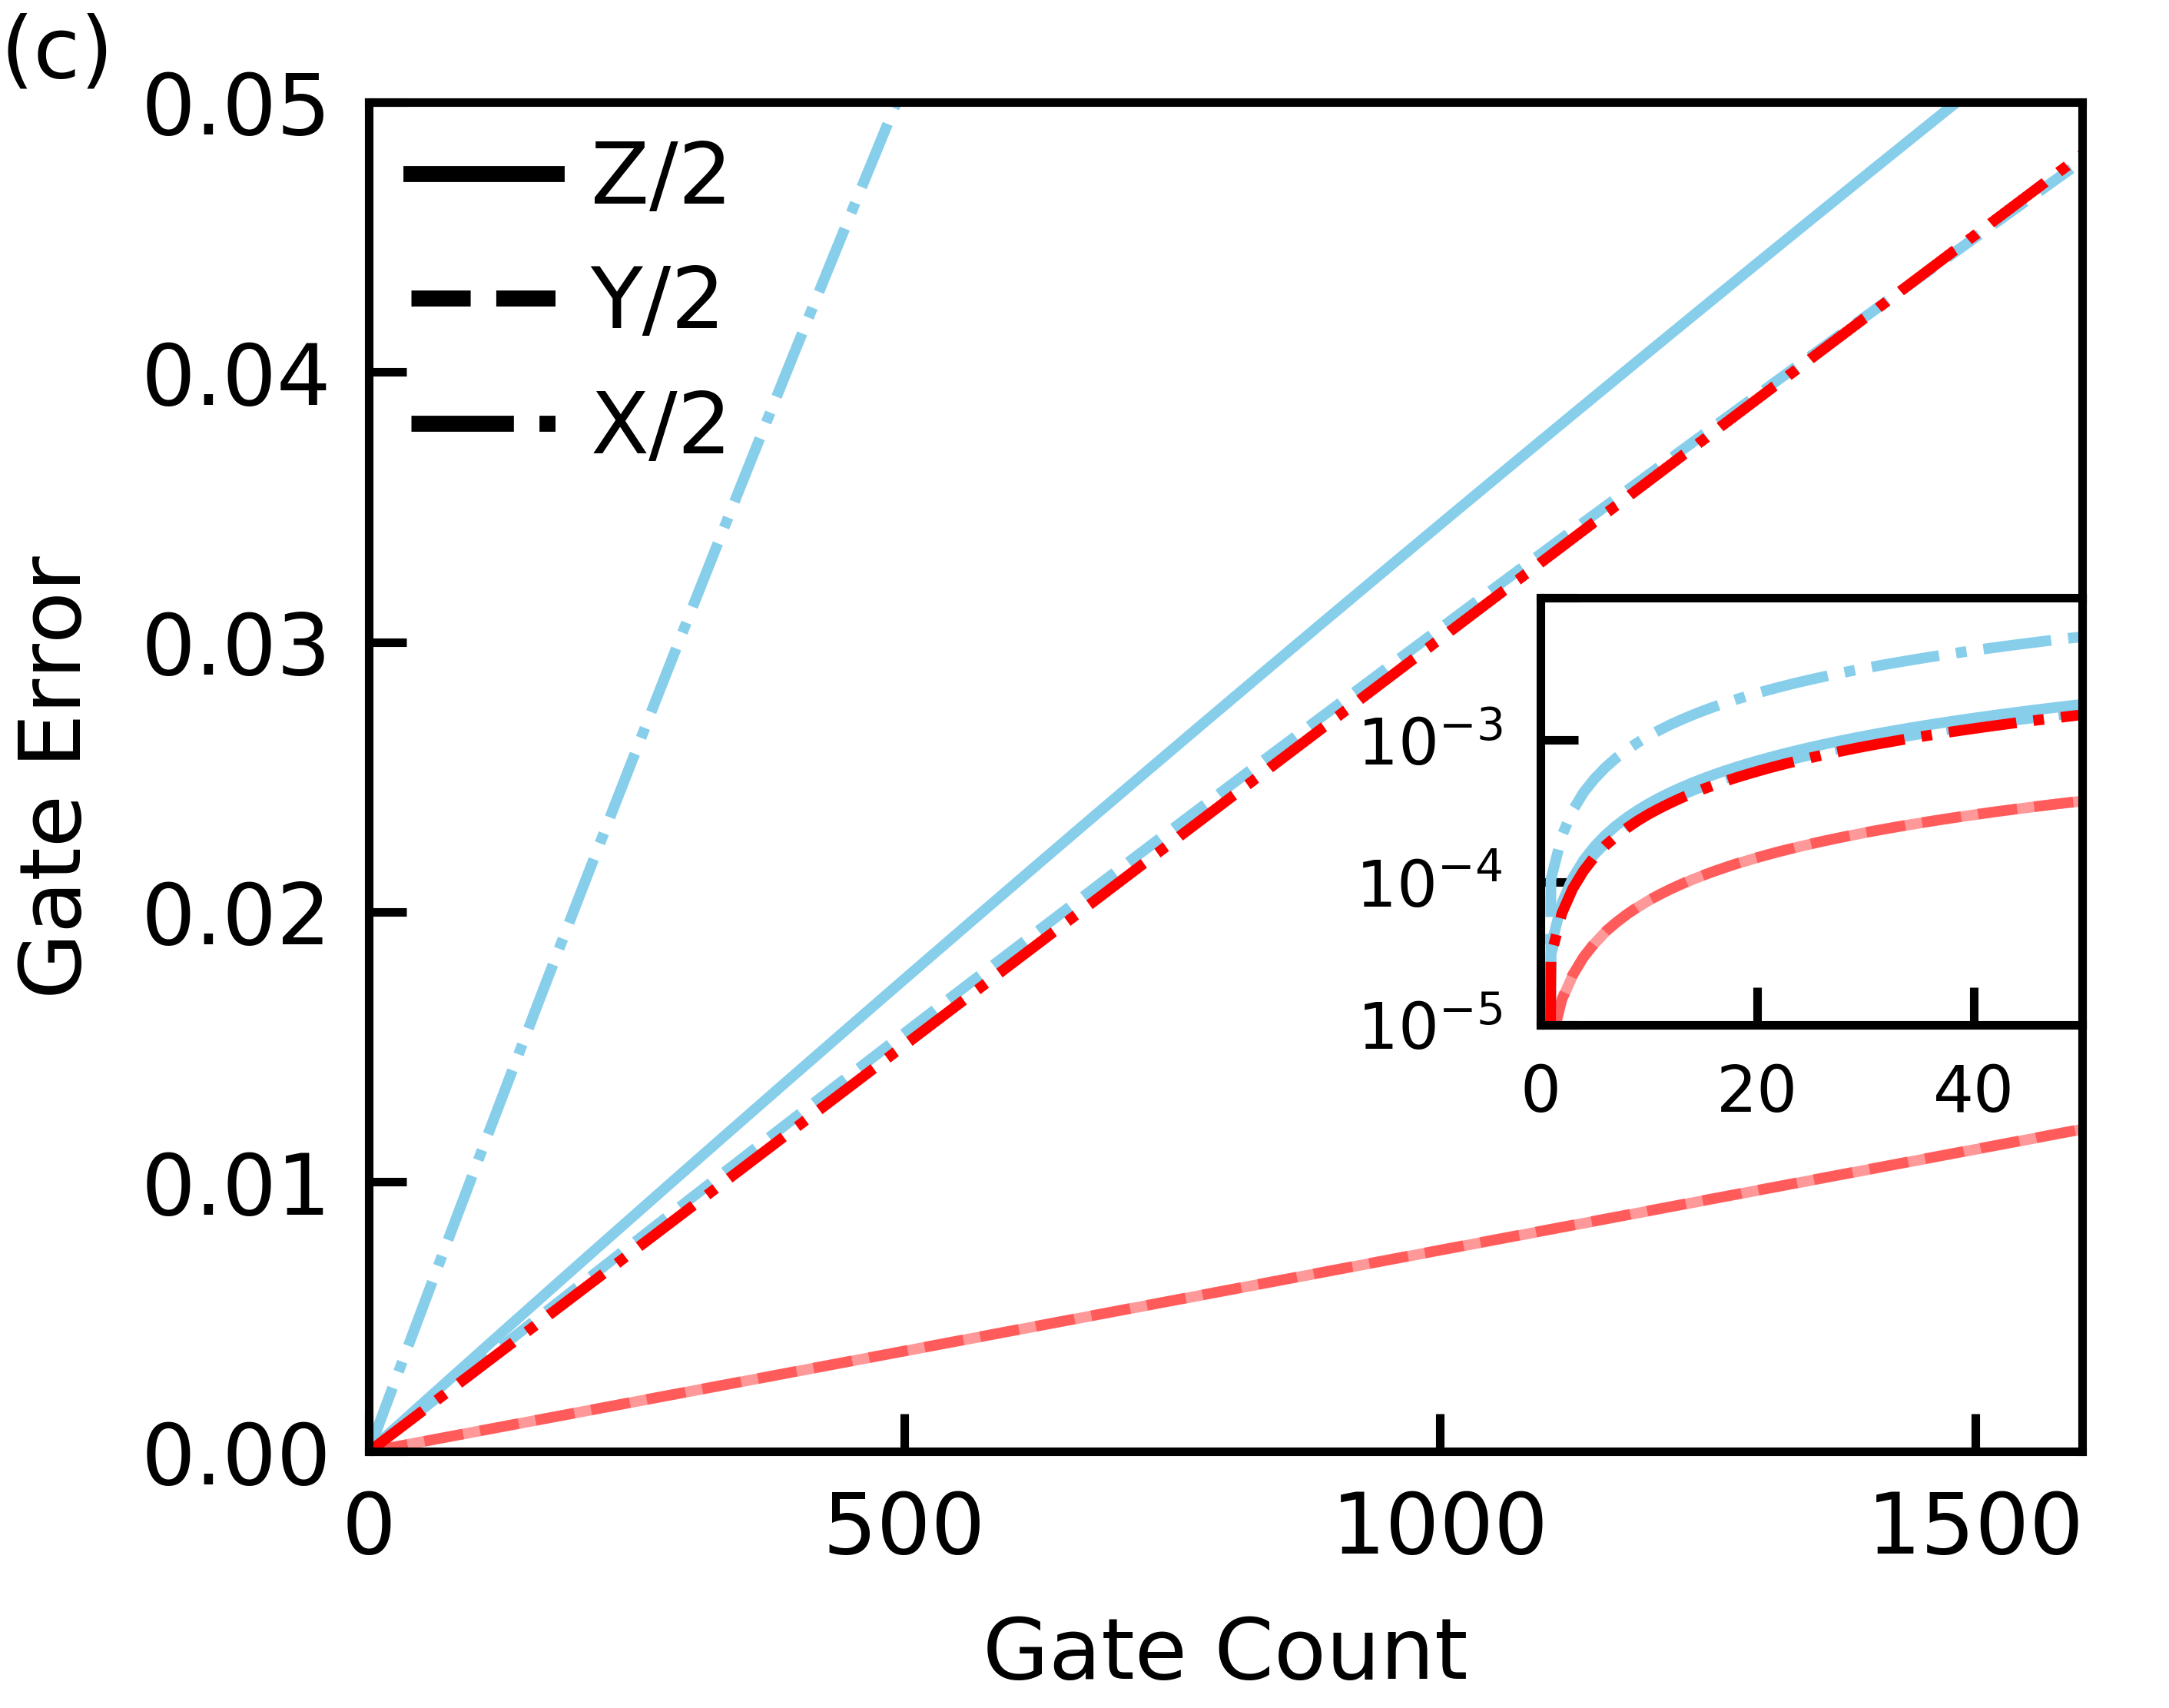
\includegraphics[width=\linewidth]{assets/f1c.png}
    \caption{\label{fig:longitudec}}
  \end{subfigure}
  \caption{
    (a) Flux pulses for the numerical gates (dark blue)
    and the analytic gates (light pink).
    (b) $T_{1}$ interpolation function used in optimization. Circle markers
    indicate measured $T_{1}$ times. Non-circle markers
    are plotted at the time-averaged 
    absolute flux and the time-averaged $T_{1}$ time for each pulse.
    (c) Cumulative gate errors due to depolarization as a function of the
    number of gates applied.
    Cumulative gate errors for the numerical $Z/2$ and $Y/2$ gates
    are indistinguishable. Inset shows log-scaled cumulative gate errors
    for small gate counts.
  }
  \label{fig:longitude}
\end{figure*}

\section{Depolarization Mitigation\label{sec:longitude}}
In this section, we outline a method
for optimizing the flux to mitigate depolarization.
For many superconducting circuits, the depolarization time
$T_{1}$ is independent of the control parameters,
so the fastest possible gate incurs the least depolarization error
\cite{schulteherbruggen2011optimal}.
For the fluxonium, however, $T_{1}$ is strongly dependent on the flux.
We enable the optimizer to trade longer gate times
for longer $T_{1}$ times, or shorter $T_{1}$ times for shorter gate times,
by making the gate time a decision variable.
Additionally, previous work has modeled the gate error due to depolarization
by evolving density matrices under a master
equation \cite{rembold2020introduction, schulteherbruggen2011optimal},
or evolving a large number of states in a quantum trajectory approach
\cite{abdelhafez2019gradient}.
We avoid the increase in computational complexity required for these
techniques by penalizing the integrated depolarization rate in optimization.

The integrated depolarization rate is given by,
\begin{equation}
  D_{1}(t) = \int_{0}^{t} T_{1}^{-1}(a(t^{\prime})) dt^{\prime}.
\end{equation}
For the gates we consider here, where the gate time is small compared to $T_{1}$,
the integrated depolarization rate is proportional to the probability of a depolarization event.
Additionally, the integrated depolarization rate is a reasonable proxy for the gate error incurred
because depolarization errors are incoherent--they increase monotonically in time without interference.
The integrated depolarization rate is appended to the augmented state \eqref{eq:astatecontrols}
and its norm is penalized in the objective \eqref{eq:costfun} by setting
the corresponding element of the target augmented state to zero.
$T_{1}(a_{k})$ is obtained at each time step by evaluating
a spline fit to experimental data of the form $\{(a, T_{1})\}$,
see Figure \ref{fig:longitudeb}.

Additionally, a master equation approach would require adding
density matrices of size $n \times n$
to the augmented state, and a quantum trajectory approach
would require adding many states of size $n$ to the augmented state,
where $n$ is the dimension of the Hilbert space.
The integrated depolarization rate is a single
real number; thus, the computational complexity of this
depolarization model does not scale
with the dimension of the Hilbert space.

We allow the optimizer to tune the gate time by
making the duration between time steps
a decision variable \cite{howell2019altro}. 
The square root of the duration $\sqrt{\Delta t_{k}}$
is appended to the augmented control \eqref{eq:astatecontrols}
and its square $\lvert \Delta t_{k} \rvert$ is used
for integration in the discrete dynamics function \eqref{eq:dyn_con},
which ensures positivity in the event that
the optimizer assigns a negative value to $\sqrt{\Delta t_{k}}$.
Further, we constraint the minimum and maximum value of the
duration to ensure integration accuracy.

We analyze the effect of depolarization on
the $X/2$, $Y/2$, and $Z/2$ gates obtained with
our numerical method and the corresponding analytic gates presented in \cite{zhang2020universal}.
We use the Lindblad master equation to simulate $T_{1}$ dissipation for successive
gate applications, and compute the cumulative gate error
after each application, see Appendix \ref{appendix:longitude}.
The gate error reported in this text is the infidelity
of the evolved state and the target state averaged over 1000 pseudo-randomly
generated initial states.

The flux pulses for the numerical gates
are approximately periodic
with amplitudes $\sim 0.2 \textrm{GHz}$, see Figure \ref{fig:longitudea}.
They are reminiscent of the analytically determined Floquet operations
for a fluxonium described in \cite{huang2020engineering}
and realized in \cite{mundada2020floquet}.
The numerical gate times are greater
than the analytic gate times, but the
numerical flux pulses
spend more time at higher flux values, achieving higher $T_{1}$ times on average,
see Figure \ref{fig:longitudeb}.
The single gate errors for both the analytic and numerical gates are
less than $10^{-4}$, which makes them sufficient for quantum error correction--a
prerequisite for fault-tolerant quantum
computing \cite{aharonov2008fault, knill2005quantum, gottesman1997stabilizer}.
However, the numerical gates achieve single gate errors
$\sim 5$ times less than those for the analytic gates,
which tracks closely with their relative improvement
on the integrated depolarization rate metric, see Appendix \ref{appendix:longitude}.
This single gate error advantage corresponds to a
significant reduction in error correction resources
\cite{paetznick2014resource, suchara2013comparing}.
Furthermore, for successive gate applications,
the gate error due to depolarization is approximately linear
in the gate count, which we expect for $t \ll T_{1}$, see Figure \ref{fig:longitudec}.
The gate error reduction for large gate counts is
important for noisy, intermediate-scale quantum (NISQ)
applications. These improvements are significant for the constraints
we have imposed on the gates,
and do not represent a fundamental limit to the optimization
methods we have employed.

